\documentclass{mcmthesis}
\usepackage{indentfirst}
\setlength{\parindent}{2em}
\mcmsetup{CTeX = true,
	tcn = 1919828
	, problem = C,
	sheet = true, titleinsheet = true, keywordsinsheet = true,
	titlepage = true, abstract = true}
\usepackage{palatino}
\usepackage{lipsum}
\usepackage{subfigure}
\title{The \LaTeX{} Template for MCM Version \MCMversion}
\author{}
\date{\today}
\begin{document}
\begin{abstract}
	fhakfhw
	\begin{keywords}
		keyword1; keyword2
	\end{keywords}
\end{abstract}
\maketitle
\tableofcontents

\newpage
\section{Introduction}

\subsection{Background}
About 275 million people worldwide, which is roughly 5.6 per cent of the global population aged 15–64 years, used drugs at least once during 2016. Some 31 million of people who use drugs suffer from drug use disorders, meaning that their drug use is harmful to the point where they may need treatment. Initial estimations suggest that, globally, 13.8 million young people aged 15–16 years used cannabis in the past year, equivalent to a rate of 5.6 per cent. 
Roughly 450,000 people died as a result of drug use in 2015, according to WHO. Of those deaths, 167,750 were directly associated with drug use disorders (mainly overdoses). The rest were indirectly attributable to drug use and included deaths related to HIV and hepatitis C acquired through unsafe injecting practices.

Opioids continued to cause the most harm, accounting for 76 per cent of deaths where drug use disorders were implicated. PWID — some 10.6 million worldwide in 2016 — endure the greatest health risks. More than half of them live with hepatitis C, and one in eight live with HIV.The headline figures for drug users have changed little in recent years, but this stability masks the striking ongoing changes in drug markets. Drugs such as heroin and cocaine that have been available for a long time increasingly coexist with NPS and there has been an increase in the non-medical use of prescription drugs (either diverted from licit channels or illicitly manufactured).The use of substances of unclear origin supplied through illicit channels that are sold as purported medicines but are destined for non-medical use is also on the increase. The range of substances and combinations available to users has never been wider. 

In 2015 and 2016, for the first time in half a century, life expectancy in the United States of America declined for two consecutive years. A key factor was the increase in unintentional injuries, which includes overdose deaths. In 2016, 63,632 people died from a drug overdose in the United States, the highest number on record and a 21 per cent increase from the previous year. This was largely due to a rise in deaths associated with pharmaceutical opioids, including fentanyl and fentanyl analogues. This group of opioids, excluding methadone, was implicated in 19,413 deaths in the country, more than double the number in 2015. It is necessary for us to study the law of drug spread and take corresponding measures to curb the trend of drug spread.\cite{1}

\subsection{Our Work}


\section{Assumptions and Notations}

\subsection{Assumptions}
We make the following basic assumptions in order to simplify the problem. Each
of our assumptions is justified and is consistent with the basic fact.
\begin{itemize}
	\item \textbf{The reported counts contains all the cases of drug use in the states and counties.} There is no unreported drug use case and the report will not lead to a reduction in drug use.
	\item \textbf{The total population of the states and counties remains essentially stable in these years.} The effect of population density on drug use cases is constant.
	\item \textbf{The rest of America and the rest of the world have a constant impact on the five states.} We assume that the external influence on these five states remains the same.
	\item \textbf{States and counties have stable policies on drug use.} We assume that policy does not change during the study period.
\end{itemize}

\subsection{Notations}
The notation table [\ref{table-notations}] contains all the notations we use in this paper.

\begin{table}[h]
	\centering
	\caption{The data example} \label{table-notations}
	\begin{tabular}{cp{20em}}
		\toprule
		ID & 28221526017700008\\
		\hline
		Time & 2018-02-28 22:15:26\\
		\hline
		PayMethod & Cash\\
		\hline
		Price & [0.982] Unit [Hainan Cherry Tomatoes] as [Season Fruit], Origin price [12.90] Discount Price [12.90]\\
		\hline
		isVip & False\\
		\hline
		SolderId & Merchant 22\\
		\bottomrule
	\end{tabular}
\end{table}

\section{Related Knowledge}

\subsection*{Graph Theory}
In \textbf{Part 1}, we need to describe the spread of the reported cases and identify possible locations where specific opioid use started. From aticle\cite{2}, we learn that weighted directed graph can solve this problem well. The advantage of using graph theory analysis is that it can directly reflect that interaction between the counties and it helps to analyze the path of transmission of certain drugs. Based on the linkages between the counties and counties, it is easier to derive strategies for controlling drug spread.

The following is the weighted directed graph we constructed. In this diagram [\ref{graph}], each node represents a county and the directed edge W$_{C,D}$ between two nodes C and D represents the influence coefficient of county C on county D is W$_{C,D}$ (The larger the influence coefficient, the more likely the county to be in county c, and the more likely the drug use in county D is to be transmitted from county C). Thus, a graph is constructed for all counties in the five states.
\begin{figure}[h]
	\centering
	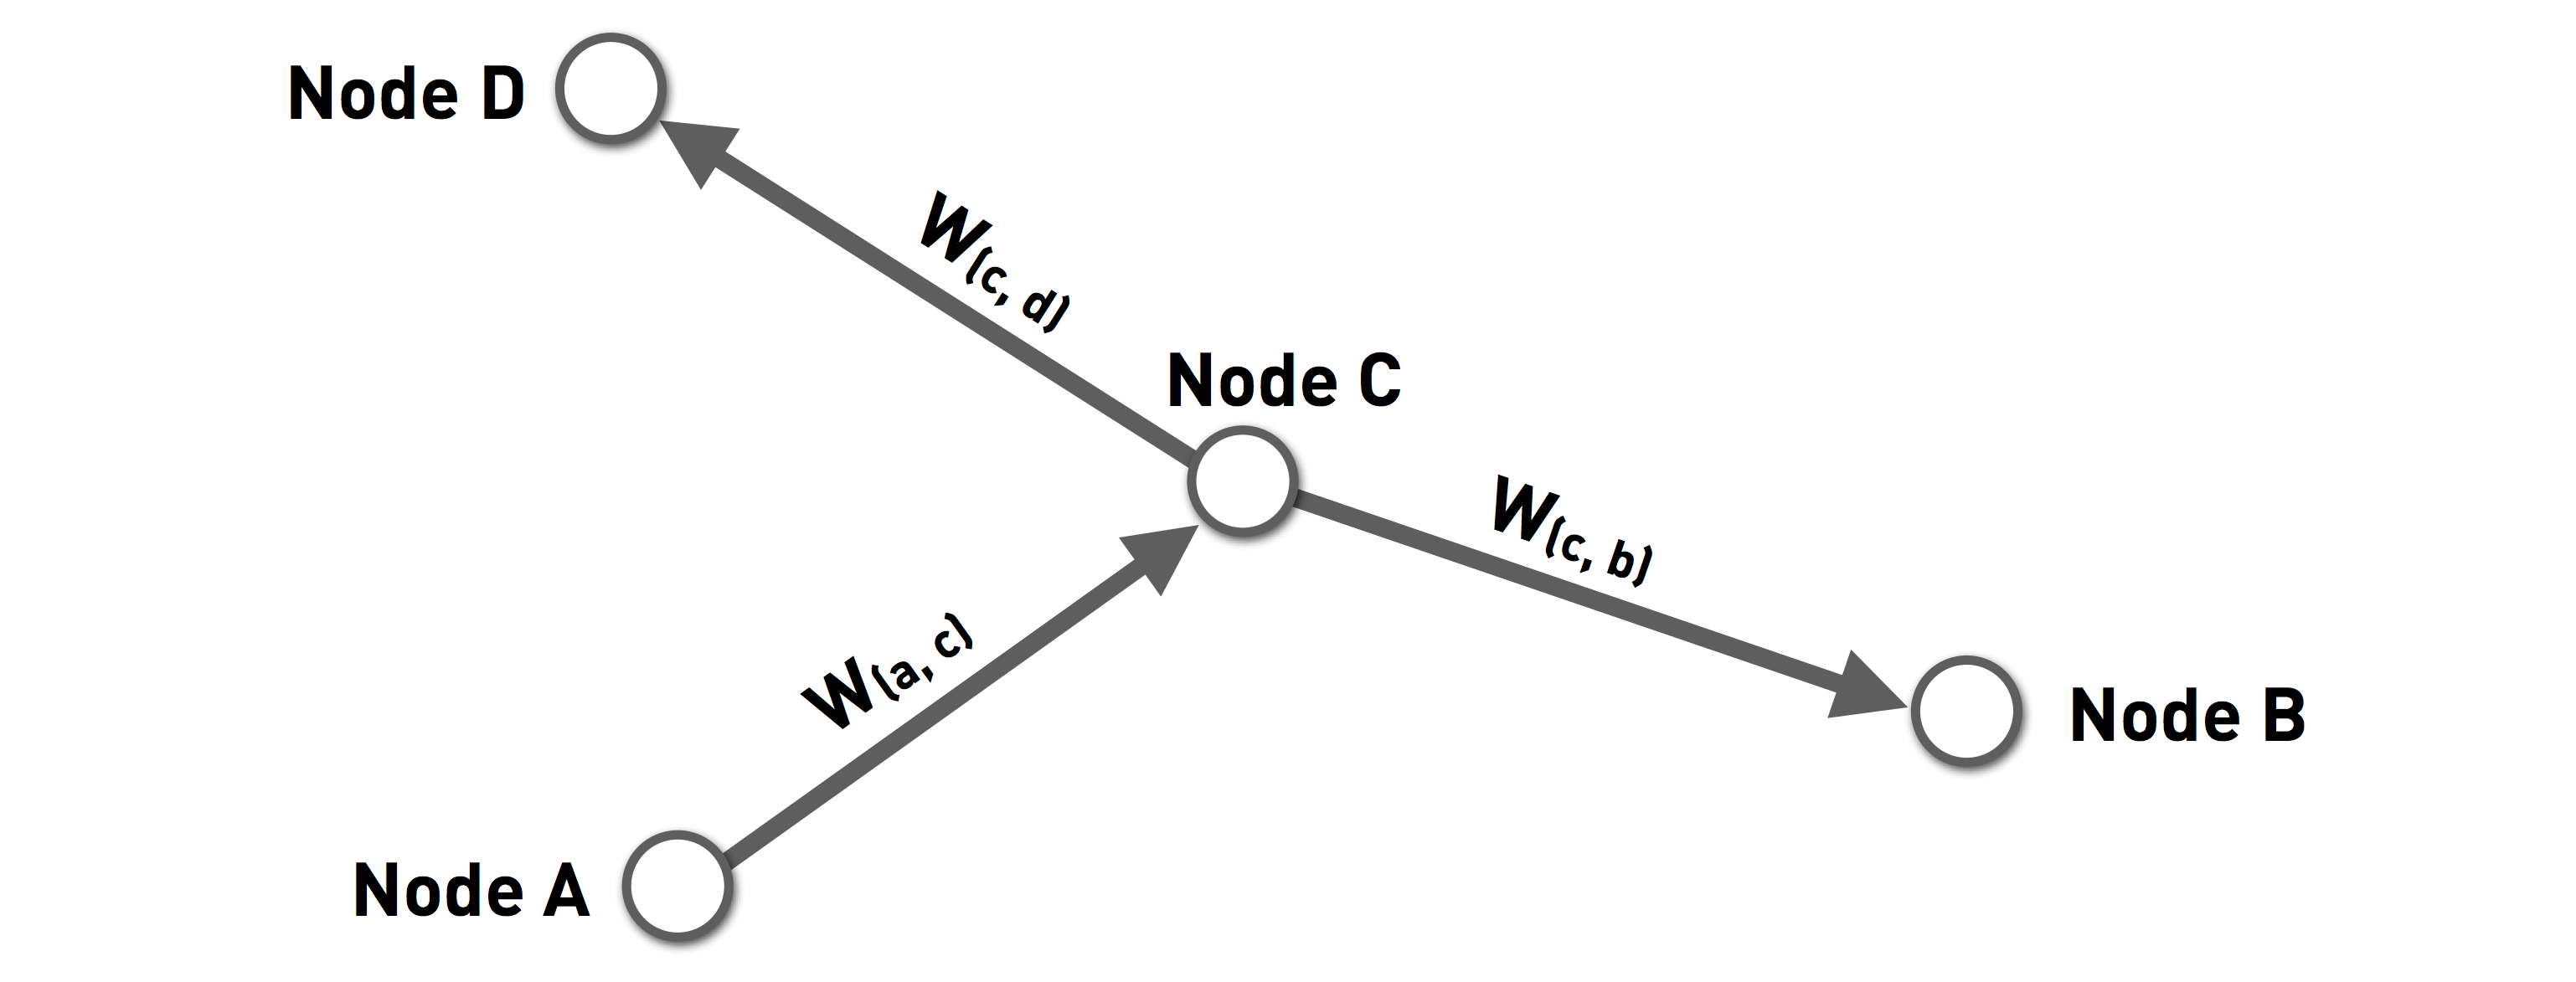
\includegraphics[width=15cm]{graphtheory.png}
	\caption{An Example of the Weighted Directed Graph}\label{graph}
\end{figure}

\section{Data Analysis}

\subsection{Data Origin}
The major data source is the ``MCM\_NFLIS\_Data.xlsx`` file. It contains all incidents involved with narcotic analgesics and heroin occurring from 2010 to 2017. Hopefully it can figure out the drug crisis spreading amount the northeast U.S.

\subsection{Obvious Factors}
Some factors are provided directly and can be grabbed at the first time:
\begin{itemize}
	\item \textbf{Substances of Drugs}\\
	The main substances of all incidents were provided, hence we may separately analyze them to validate the model.
	\item \textbf{Case Count}\\
	Many drugs involved in all these incidents, but they are not equally significant. The reported count recording the troubles they made can be a convincing factor to determine how influential one drug is.
	\item \textbf{Geography Location}\\
	The specific county name in OH, KY, WV, VA, and PA are provided in detail. Thanks to $Simple\ Maps\ Corp.$[1] and their generous contribution, we could get accurate longitude and latitude to locate a single county. That would be a great help in visualizing our analysis.
\end{itemize}

\subsection{Error Data Fix}

\section{Model Construction and Simulation Analysis}
\subsection{Problem 1}
\subsubsection{Construction Process}
We analyze and process the data of ``MCM\_NFLIS\_Data.xlsx" and establish databases and a flow chart[\ref{sum_flowchart}] for the total number of synthetic opioid and heroin cases in 451 counties of the five states from 2010 to 2017.
\begin{figure}[ht]
	\centering
	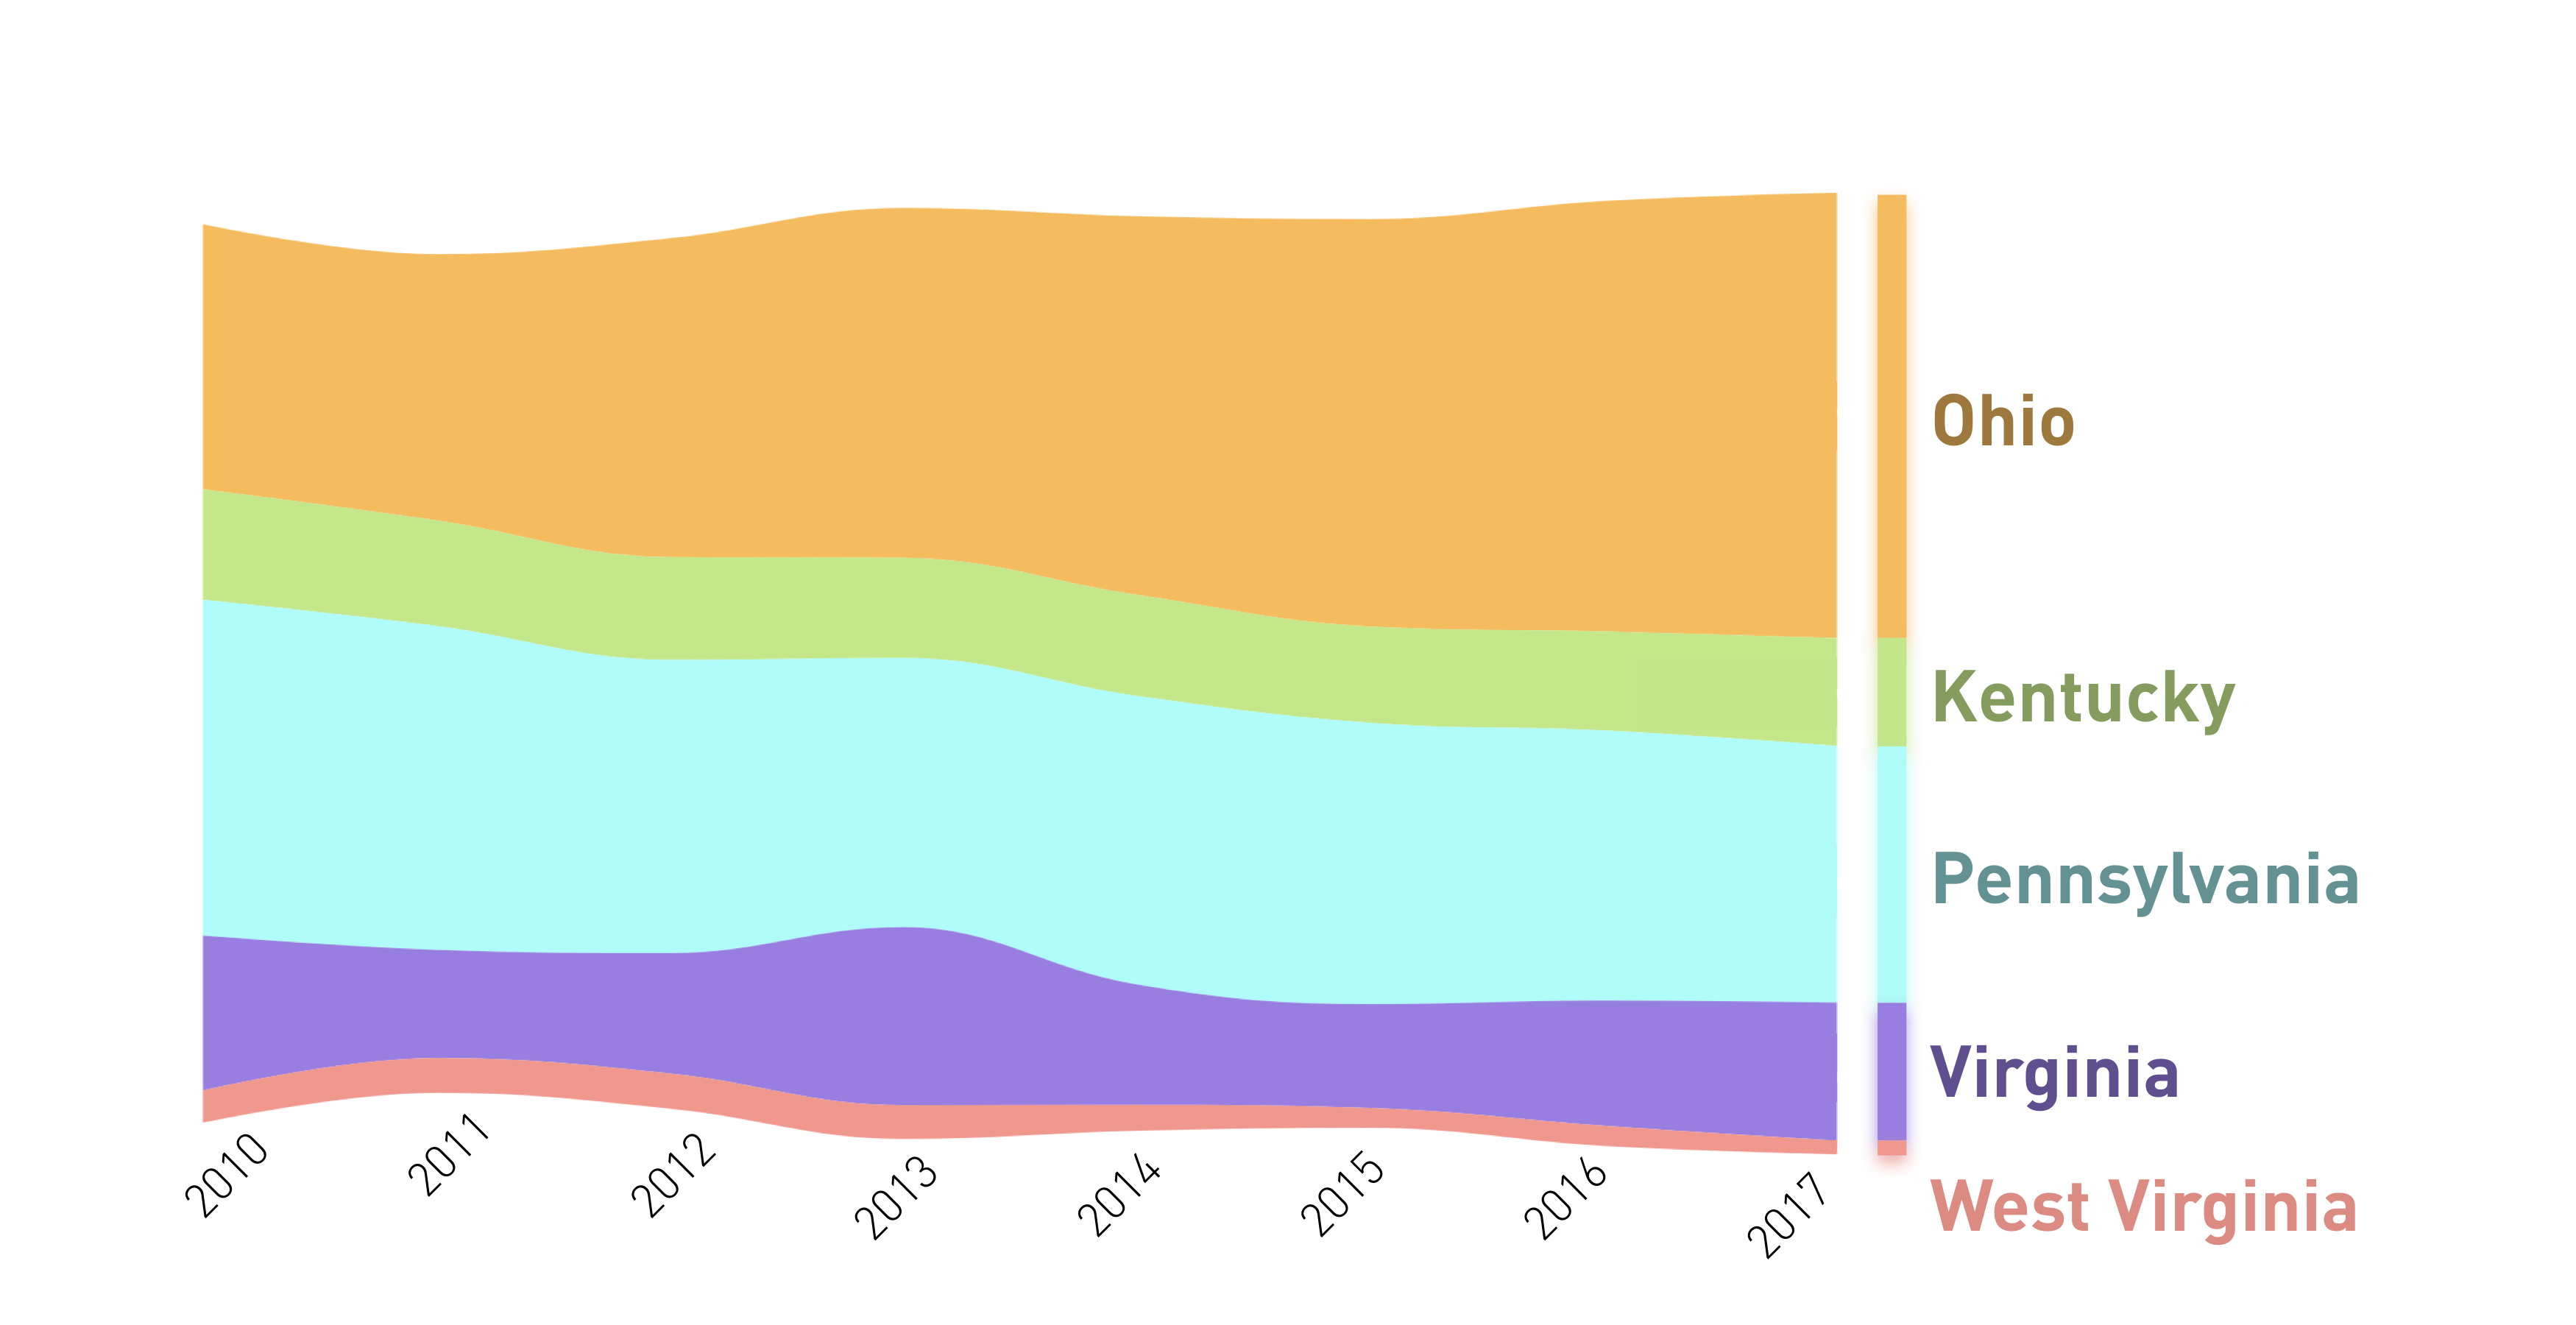
\includegraphics[width=15cm]{StateSum.png}
	\caption{Total Drug Use In Five States in Years 2010-2017}\label{sum_flowchart}
\end{figure}

Through the overall analysis of the flow chart, we find that the number of cases has a tendency to rise slowly. We take the following steps to build this model.First of all, we think that the change in the number of cases in a county $Y(t)$ depends on two factors: time $T(t)$ and space $S(t)$ and these two factors have equally important influence on the change of the case number. Based on this, the space-time model of $Y(t) = T(t)S(t)$ type for the county case number is established:
\begin{enumerate}
	\item \textbf{The impact of the number of local cases in the past on the present.} According to the knowledge of time series, we need $T(t)$ to reflect the trend and periodicity of case number changes. Therefore, $T(t)$ should be a component that fluctuates slowly with time. We assume that $ T(t) = C_{base}e^{sin(\omega t+\varphi)}$, where $C_{base}$ is the base level of the number of cases in the county, $\omega$ in $e$ is the angular velocity of the number of cases in the county, and $\varphi$ is the modified initial phase.
	\item \textbf{The influence of the number of cases in the current space around on the number of local cases.} According to the figure we establish, we need $S(t)$ to reflect the randomness and correlation of the number of cases, so $S(t)$ should be a random component monitoring the influence of the number of cases in the surrounding space. We believe that the impact on the number of the cases in the local counties is positively correlated with the number of the adjacent county cases and negatively correlated with the distance between the two places. At the same time, we note that distance and influence are not strictly inversely proportional. For example, at a distance of enough, a difference of 1 or 2 kilometers does not make a significant difference. We think that taking the logarithm of the distance is going to be a good solution.
\end{enumerate} 

Based on the above, we get Equation \eqref{model1_eq1}.
\begin{equation}
P_{j}(t) = C_{base} e^{\sin (\omega t+\varphi)} (1+\sum_{i=1}^{k} {\frac{C_{i,j} P_{i}(t)}{\ln (D_{i,j}+1)}})
\label{model1_eq1}
\end{equation}

In the equation, $P_{j}$ represents the number of cases in the target county, $P_{i}$ represents the number of cases in the surrounding county, $(1+\sum_{i=1}^{k} {\frac{C_{i,j} P_{i}(t)}{\ln (D_{i,j}+1)}})$ represents the effect of $k$ surrounding counties on target counties (We consider that this parameter is going to be the value of fluctuating on a base of $1$), $C_{i,j}$ represents the influence coefficient of county i on county j, and $D_{i,j}$ represents the distance between county i and county j.

\subsubsection{Model Simplification}
In the model, if we take into account the relationship among all counties, then $k$ will be 451, and we will calculate 451 correlation coefficients when we analyze each county. Considering that there is the data of only eight years from 2010 to 2017 in the file ``MCM\_NFLIS\_Data.xlsx``, we cannot specifically calculate the specific value of each parameter. And when the geographical location of two counties is far from each other, the relationship between them is relatively small, and then its influence can be ignored. In other words, we can only take adjacent counties that are close to the target county as the analysis target. How do we define proximity? Based on the map information, we collect the longitude and latitude information of each county. Since the latitude and longitude of the five states do not vary much, we used the longitude and latitude of the two locations to calculate their relative distances\eqref{distance}.
\begin{equation}
D_{i,j} = \sqrt{(lon_i-lon_j)^2+(lat_i-lat_j)^2}
\label{distance}
\end{equation}

In the equation, $lon_i$ represents the longitude of county $i$, $lon_j$ represents the longitude of county $j$, $lat_i$ represents the latitude of county $i$, and $lat_i$ represents the latitude of county $i$. For each county, we rank the surrounding counties from smallest to largest by distance. How many surrounding counties should we choose? From article\cite{}, we learned that using variance and bias analysis can help us get the right parameter $k$. We get Figure \ref{model1_bias_variance} as a result. From the figure, when $k = 3$, we can get the best fit.
\begin{figure}[ht]
	\centering
	\subfigure[Bias Analysis]{
		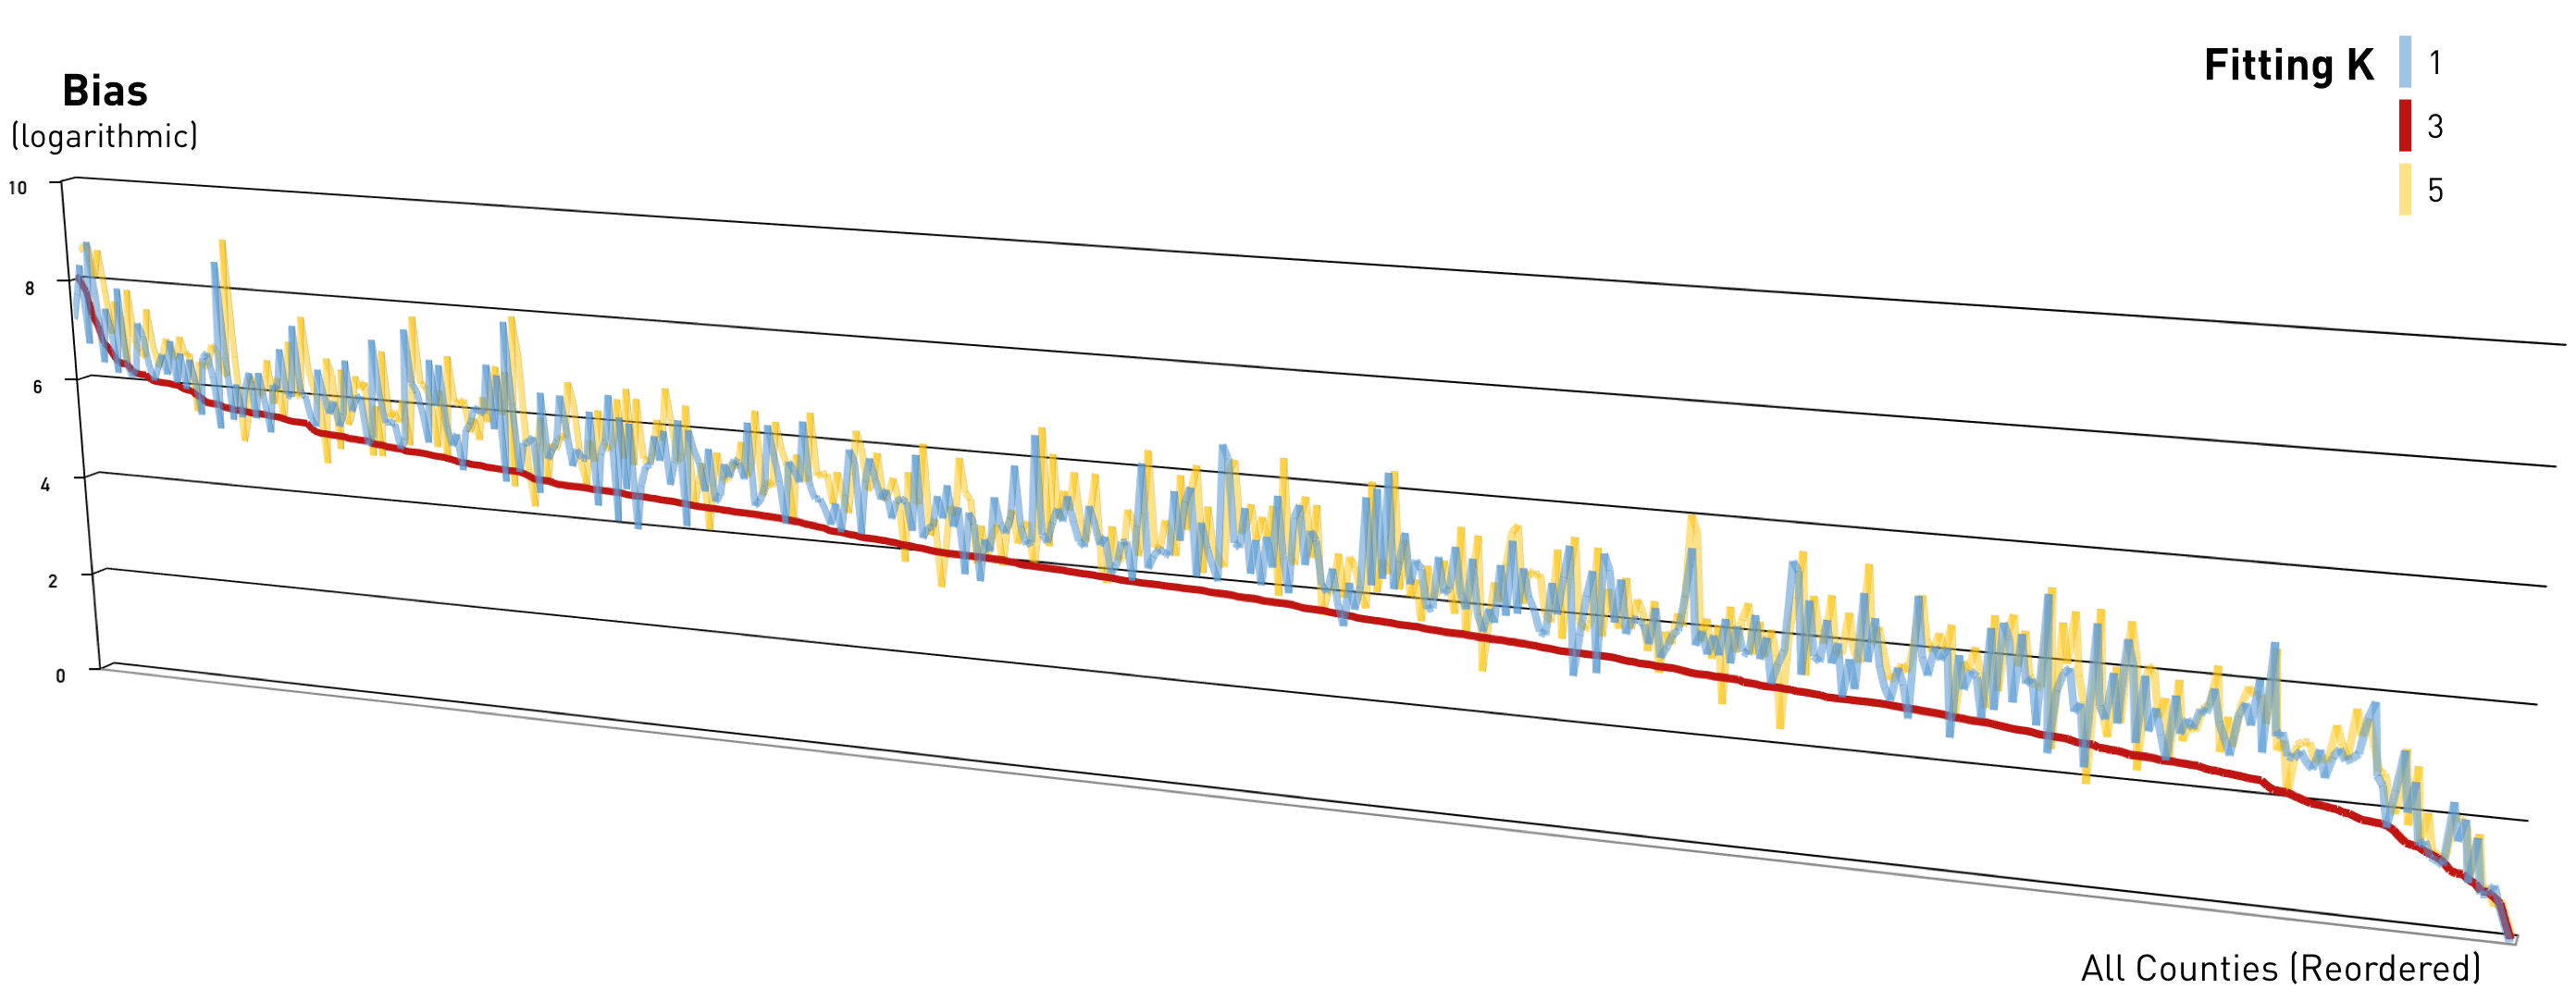
\includegraphics[width=15cm]{model1_bias}\label{model1_bias}
	}
	\subfigure[Variance Analysis]{
		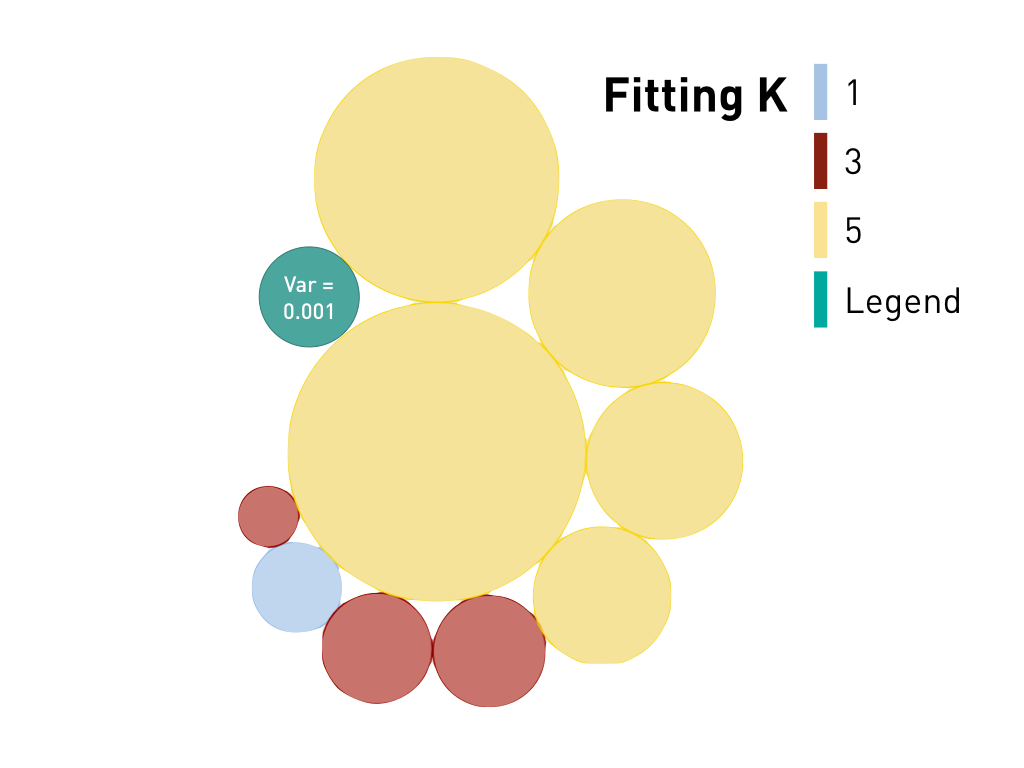
\includegraphics[width=8cm]{model1_variance}\label{model1_variance}
	}
	\caption{Bias And Variance Analysis}\label{model1_bias_variance}	
\end{figure}

Finally, we can get the simplified equation\eqref{model1_sim}:
\begin{equation}
P_{j}(t) = C_{base} e^{\sin (\omega t+\varphi)} \left(\frac{C_1 P_1(t)}{\ln (D_1+1)}+\frac{C_2 P_2(t)}{\ln (D_2+1)}+\frac{C_3 P_3(t)}{\ln (D_3+1)}\right)
\label{model1_sim}
\end{equation}
\subsubsection{Problem Solving}
Based on Equation\eqref{model1_sim}, we put the data of eight years into the formula to fit it, and we get a graph of each county based on the total amount of drugs\ref{all_relation}.
\begin{figure}[ht]
	\centering
	\includegraphics[width=15cm]{all_relation.png}
	\caption{}\label{all_relation}
\end{figure}



\subsubsection{Sensitivity Analysis}

\subsection{Problem 2}
\subsubsection{Construction Process}
In this problem, we develop the model in Problem 1, and use the modified model as a tool to probe into the problem with the analytic hierarchy process. First, we consider a problem from the bottom up. We analyze and process the data in the ``ACS\_1x\_5YR\_DP02" folder, and find that they divide the county's demographics and family structure by different criteria. Then we establish a structural proportion database for each county from 2010 to 2017. These indicators are grouped into three categories: family factors, educational factors, and cultural factors and the structure of each indicator is divided into influential factors and non-influential factors\ref{model2_layer}. For example, in the education level indicator, we consider that people with high school education and below account for the majority of cases, while those with higher levels of education account for the minority. After this division, we do the geometric average on the indicator to get the criterion of a category. Inside criterion, each indicator has the same weight.
\begin{figure}[h]
	\centering
	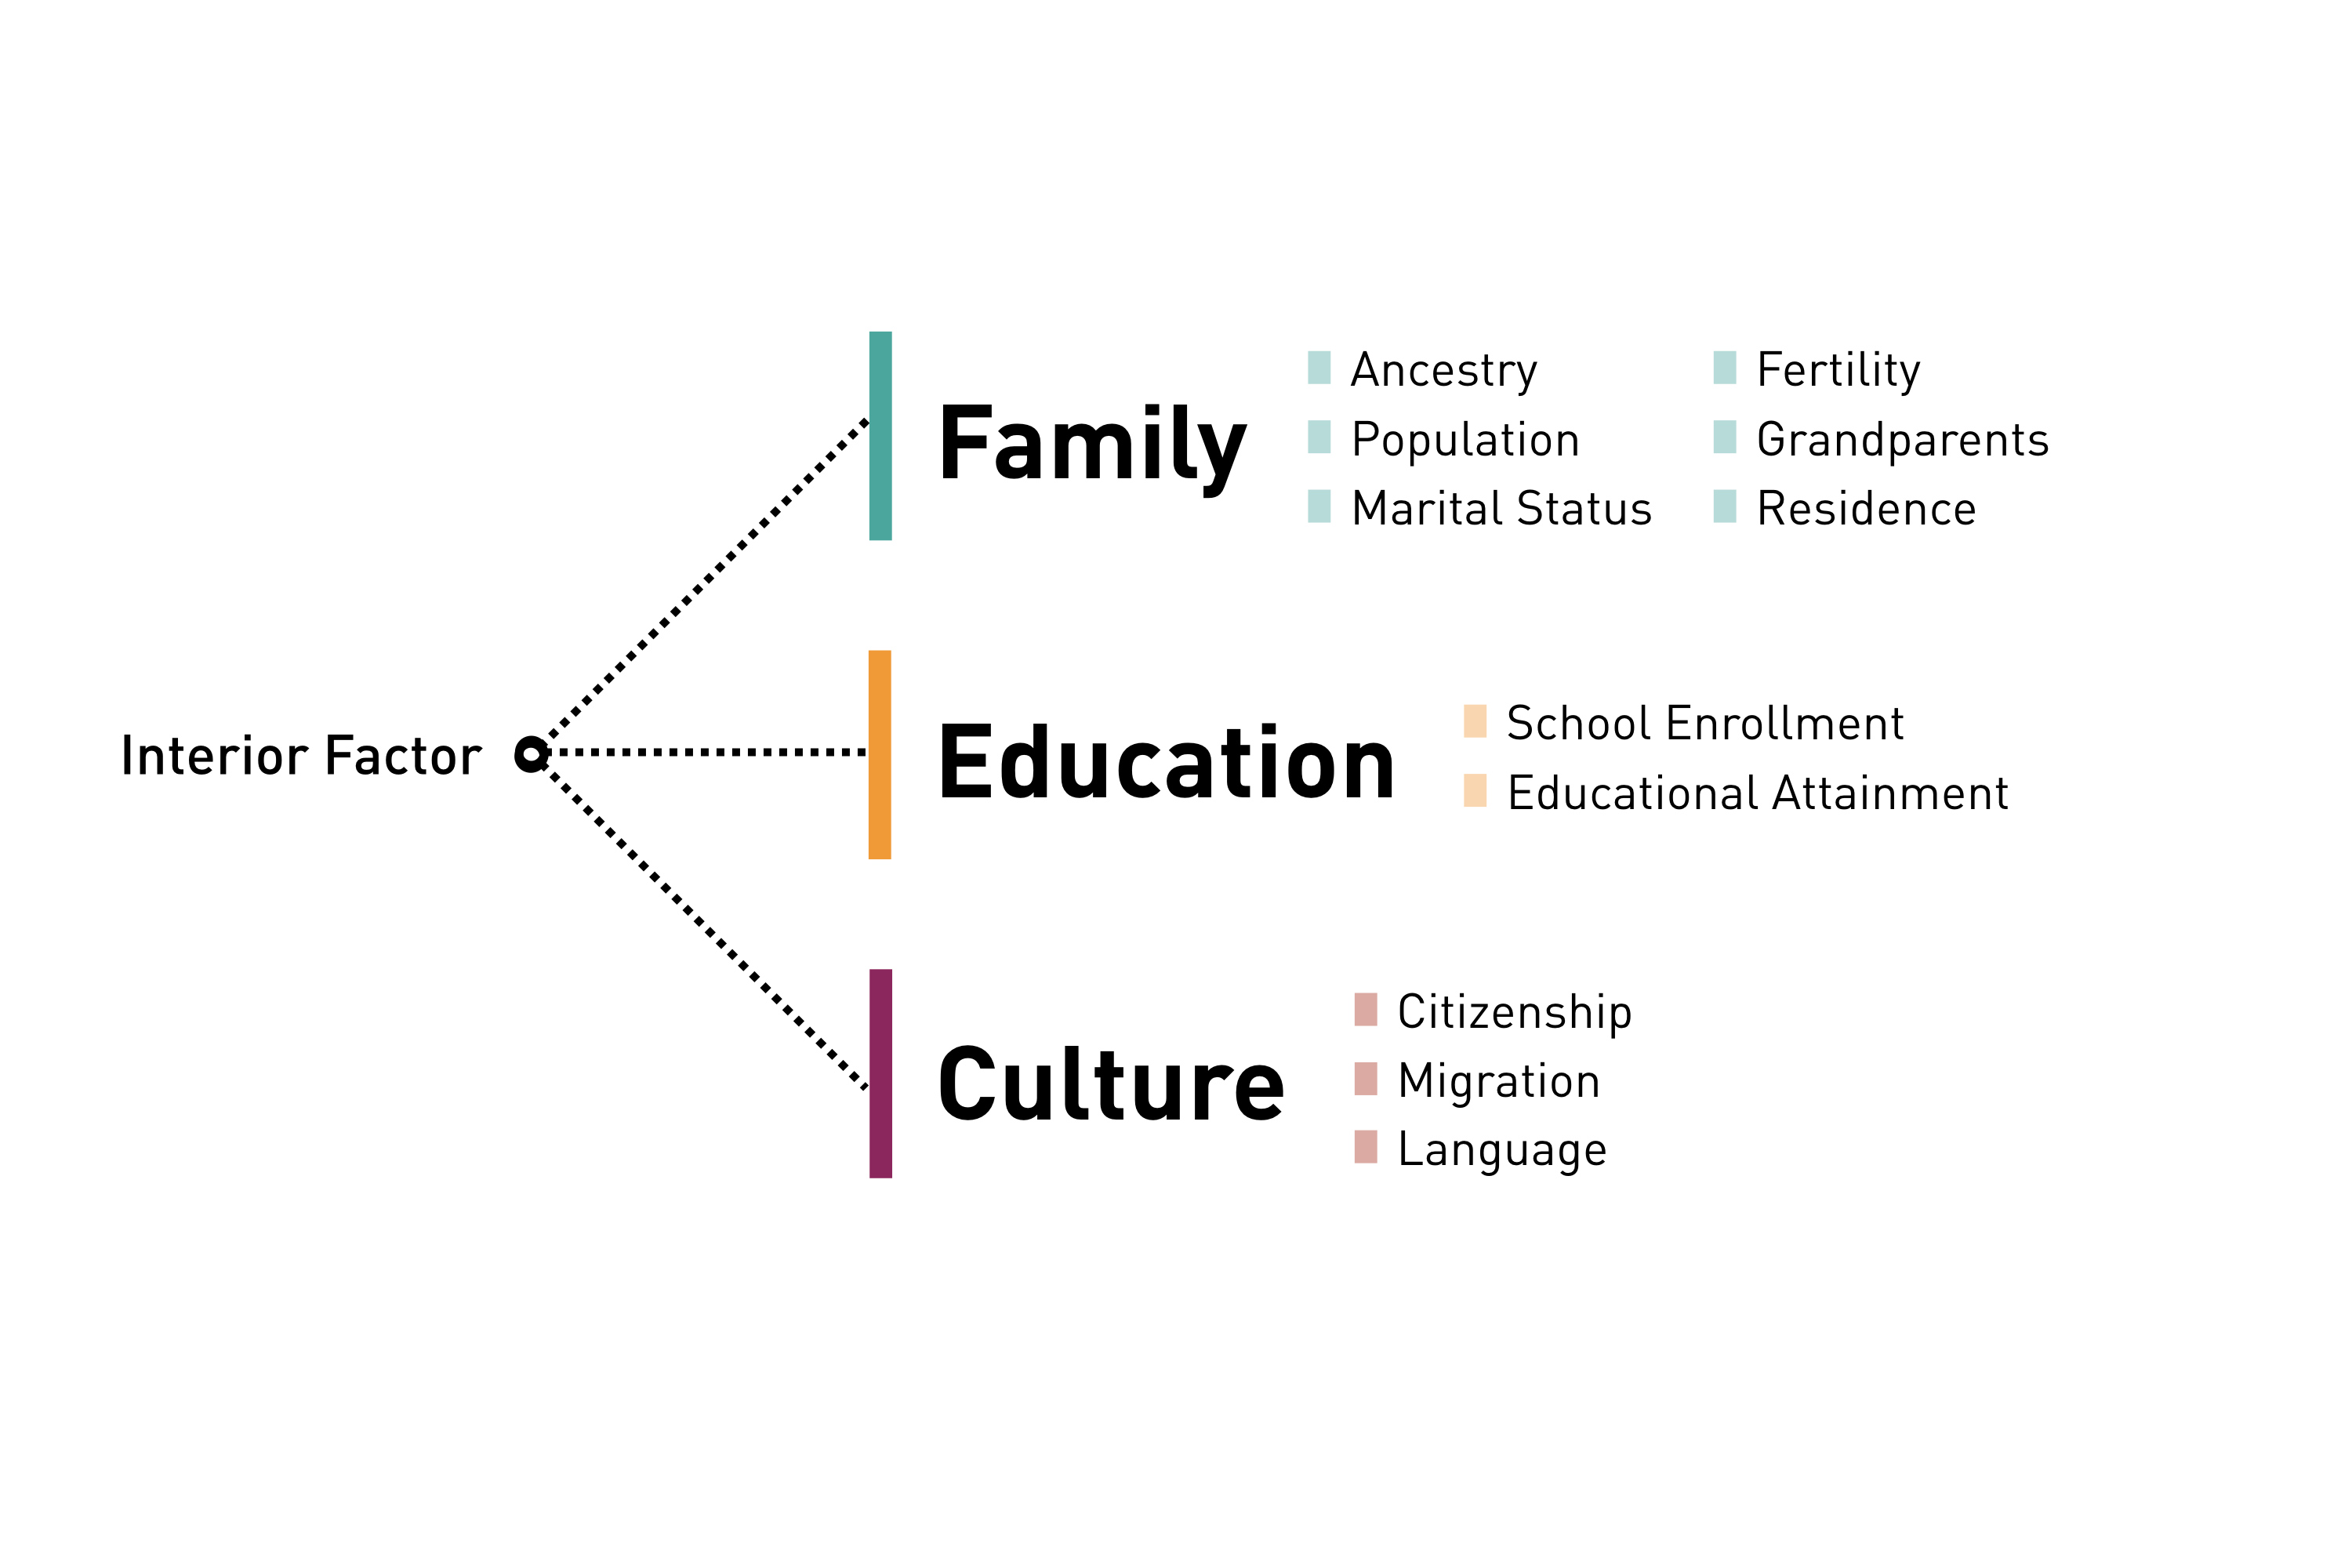
\includegraphics[width=15cm]{model2_layer.png}
	\caption{AHP of Factors Affecting Drug Use}\label{model2_layer}
\end{figure}

Secondly, we fit the model from the top down. We use the control variable method to study the importance of family factors to educational factors, family factors to cultural factors, and family factors to cultural factors. The following is an example of the importance of the education factor to the family factor of a county. We assume that family factor is $F$, educational factor is $E$, the degree of importance is $x$. We add $\left( F\*x+E\right) $ as a coefficient to model one and get Equation \eqref{model2_eq1}. After fitting, we can get the value of $x_{F,E}$.
\begin{equation}
P_{j}(t) = C_{base} e^{\sin (\omega t+\varphi)} \left(\frac{C_1 P_1(t)}{\ln (D_1+1)}+\frac{C_2 P_2(t)}{\ln (D_2+1)}+\frac{C_3 P_3(t)}{\ln (D_3+1)}\right)\left( F\*x+E\right)
\label{model2_eq1}
\end{equation}

And so on we can get three important levels($x_{F,E}$, $x_{F,C}$, $x_{E,C}$) for each county. And then we can get the following matrix.

\[
\begin{pmatrix}
{1 } & {x_{F,E} } & {x_{F,C} }  \\
{\frac{1}{x_{F,E}}} & {1 } & {x_{E,C} }  \\
{\frac{1}{x_{F,C} } } & {\frac{1}{x_{E,C}} } & {1}  \\
\end{pmatrix}
\]

A new matrix is obtained by normalizing each column of the matrix. Then we figure out the average value of each row, and they are influence coefficients of family factor, education factor and cultural factor of each county ($a$,$b$, and $d$). Finally taking the logarithm of the population of each county, we take the weighted average of the three coefficients and get The general coefficients of the three influence factors. We get the final equation: Equation\eqref{model2_eq2}.
\begin{equation}
P_{j}(t) = C_{base} e^{\sin (\omega t+\varphi)} \left(\frac{C_1 P_1(t)}{\ln (D_1+1)}+\frac{C_2 P_2(t)}{\ln (D_2+1)}+\frac{C_3 P_3(t)}{\ln (D_3+1)}\right)\left(a\*F+b\*E+d\*C\right)
\label{model2_eq2}
\end{equation}

\subsection{Problem 3}
\subsubsection{Problem Solving}
In model 1, we consider that case number changes are influenced by both time and space factors and obtain the fitting result with small deviation. In model 2, we combine the results of the county population survey, focuse on the internal factors, and identify the important degree of the influence of different population factors through the analytic hierarchy process. Based on all the data provided and the county geographic information that we have looked up, we can get a complete equation\eqref{model2_eq2} of how the county case numbers are changing.

We have taken into account the response to the drug crisis in many regions and find that they take into account both the whole and the parts.

\subsection{Strengths}
\begin{itemize}
	\item \textbf{Applies widely}\\
	This  system can be used for many types of airplanes, and it also
	solves the interference during  the procedure of the boarding
	airplane,as described above we can get to the  optimization
	boarding time.We also know that all the service is automate.
	\item \textbf{Improve the quality of the airport service}\\
	Balancing the cost of the cost and the benefit, it will bring in
	more convenient  for airport and passengers.It also saves many
	human resources for the airline.
\end{itemize}

\subsection{Weaknesses}
\begin{itemize}
	\item
\end{itemize}

\section{Conclusions}


\begin{thebibliography}{99}
	\bibitem{1} ``WORLD DRUG REPORT 2018", \url{https://www.unodc.org/wdr2018/prelaunch/}
	\bibitem{2} Boccaletti S, Latora V, Moreno Y, Chavez M, Hwang D U. ``Complex networks: Structure and dynamics". Physics reports, 2006, 424(4): 175-308.
	\bibitem{3}
	\bibitem{4}\url{http://www.chinatex.org/}
\end{thebibliography}


\begin{appendices}
	
	\section{First appendix}
	
	\lipsum[13]
	
	Here are simulation programmes we used in our model as follow.\\
	
	%\textbf{\textcolor[rgb]{0.98,0.00,0.00}{Input matlab source:}}
	%\lstinputlisting[language=Matlab]{./code/mcmthesis-matlab1.m}
	
	\section{Second appendix}
	
	%some more text \textcolor[rgb]{0.98,0.00,0.00}{\textbf{Input C++ source:}}
	%\lstinputlisting[language=C++]{./code/mcmthesis-sudoku.cpp}
	
	
\end{appendices}
	
	
\end{document}
